% Standard pen-and-paper worksheet preamble.
% Compile with: xelatex -interaction=nonstopmode exercise.tex   (run twice)
\documentclass[a4paper, 14pt]{extarticle}
\usepackage[top=1in, bottom=1in, left=1in, right=1in]{geometry}
\usepackage{amsmath}
\usepackage{amssymb}
\usepackage{graphicx}
\usepackage{hyperref}
\usepackage{tcolorbox}
\usepackage{enumitem}
\usepackage{multicol}
\usepackage{adjustbox}
\usepackage{etoolbox}
\usepackage{tikz}
\usepackage{fontspec}
\usetikzlibrary{calc,decorations,patterns,arrows,decorations.pathmorphing,positioning}
\definecolor{pltblue}{HTML}{1F77B4}

% Handwriting font, resolved once into \ppfont and \ppfontname.
%
% "Pretty Neat" (xkcd-style) is the house face and is installed on almost
% nothing. Excalifont is vendored in tools/fonts/ and installed by CI, so it is
% the one face that is always present; Latin Modern is the last resort.
%
% Naming a font that is not installed is a hard error, not a fallback, which is
% why this is a chain and not a line: seven sheets used to name one outright
% and stopped building the day it was uninstalled.
\def\ppfontname{Latin Modern Roman}
\IfFontExistsTF{Pretty Neat}{\def\ppfontname{Pretty Neat}}{%
  \IfFontExistsTF{Humor Sans}{\def\ppfontname{Humor Sans}}{%
    \IfFontExistsTF{Excalifont}{\def\ppfontname{Excalifont}}{}}}
\expandafter\newfontfamily\expandafter\ppfont\expandafter{\ppfontname}
\expandafter\setmainfont\expandafter{\ppfontname}
\tikzset{every picture/.style={/utils/exec={\ppfont}}}
\AtBeginEnvironment{tabular}{\ppfont}

% xkcd-style hand-drawn line decoration.
% WARNING: applying [xkcd] to many nodes can throw "Dimension too large".
% Use it on a handful of \draw lines only, never on every node.
\makeatletter
\pgfset{
  /pgf/decoration/randomness/.initial=2,
  /pgf/decoration/wavelength/.initial=100
}
\pgfdeclaredecoration{sketch}{init}{
  \state{init}[width=0pt,next state=draw,persistent precomputation={
    \pgfmathsetmacro\pgf@lib@dec@sketch@t0
  }]{}
  \state{draw}[width=\pgfdecorationsegmentlength,
  auto corner on length=\pgfdecorationsegmentlength,
  persistent precomputation={
    \pgfmathsetmacro\pgf@lib@dec@sketch@t{mod(\pgf@lib@dec@sketch@t+pow(\pgfkeysvalueof{/pgf/decoration/randomness},rand),\pgfkeysvalueof{/pgf/decoration/wavelength})}
  }]{
    \pgfmathparse{sin(2*\pgf@lib@dec@sketch@t*pi/\pgfkeysvalueof{/pgf/decoration/wavelength} r)}
    \pgfpathlineto{\pgfqpoint{\pgfdecorationsegmentlength}{\pgfmathresult\pgfdecorationsegmentamplitude}}
  }
  \state{final}{}
}
\tikzset{xkcd/.style={decorate,decoration={sketch,segment length=0.5pt,amplitude=0.5pt}}}
\makeatother

\setlength{\parindent}{0pt}
\setlength{\parskip}{0.5em}

\begin{document}

\section*{Turning the Dial}

Ringville has grown. Twenty houses now sit around the ring, and people have
become slightly more sociable: everyone knows the \emph{two} neighbors on each
side. Nobody else.

\begin{center}
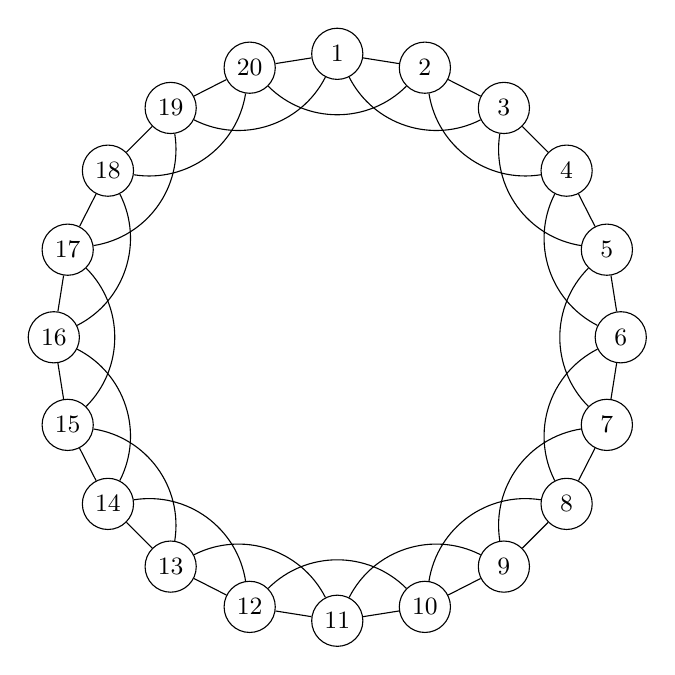
\begin{tikzpicture}[scale=1.0]
    \foreach \i in {1,...,20} {
        \node[draw, circle, inner sep=0.5pt, minimum size=6.5mm]
            (N\i) at ({90-(\i-1)*18}:3.6) {\small \i};
    }
    \foreach \i in {1,...,20} {
        \pgfmathtruncatemacro{\j}{mod(\i,20)+1}
        \pgfmathtruncatemacro{\k}{mod(\i+1,20)+1}
        \draw (N\i) -- (N\j);
        \draw (N\i) to[bend right=45] (N\k);
    }
\end{tikzpicture}
\end{center}

You now have names for everything you measured before: distance, average path
length, diameter, clustering, the random baseline, the small-world index
$\sigma$. This sheet is where you find out how much those names are worth.

\section*{Part 1: The town before anything is rewired}

{\bf Question 1}:
Measure the town as it stands.

\begin{enumerate}
    \item Write down the four people that person 1 knows:
          \underline{\hspace{5cm}}
    \item How many pairs among those four are themselves connected?
          \underline{\hspace{2cm}}

          So person 1's local clustering coefficient is
          \underline{\hspace{2cm}}
    \item Every person in this town sits at the corner of the same number of
          triangles. How many triangles does the whole town contain?
          \underline{\hspace{2cm}}

          Say in one line how you got there without drawing all of them.

          \underline{\hspace{\textwidth}}
\end{enumerate}

\begin{minipage}{\textwidth}
{\bf Question 2}:
Now distances. Instead of listing all nineteen people, use the ring: a person
$d$ houses away along the circle needs how many handshakes? Fill the top row by
walking a few examples on the drawing, then finish the row by the pattern.

\begin{center}
{\small
\begin{tabular}{|l|p{0.72cm}|p{0.72cm}|p{0.72cm}|p{0.72cm}|p{0.72cm}|p{0.72cm}|p{0.72cm}|p{0.72cm}|p{0.72cm}|p{0.72cm}|}
\hline
Houses away $d$ & 1 & 2 & 3 & 4 & 5 & 6 & 7 & 8 & 9 & 10 \\
\hline
Handshakes & & & & & & & & & & \\[0.5cm]
\hline
How many people & & & & & & & & & & \\[0.5cm]
\hline
\end{tabular}
}
\end{center}
\end{minipage}

\begin{enumerate}
    \item Average handshakes from person 1 to everyone else:
          \underline{\hspace{3cm}}
    \item Diameter of the town: \underline{\hspace{2cm}}
    \item Does the average you just computed depend on \emph{which} person you
          started from? Why?

          \underline{\hspace{\textwidth}}
\end{enumerate}

\clearpage

\section*{Part 2: One edge}

{\bf Question 3}:
Person 1 falls out with person 2 and befriends person 11 instead. So:
\textbf{erase the edge 1--2}, and \textbf{draw the edge 1--11}. The town still
has exactly forty friendships --- you moved one, you did not add one.

\begin{center}
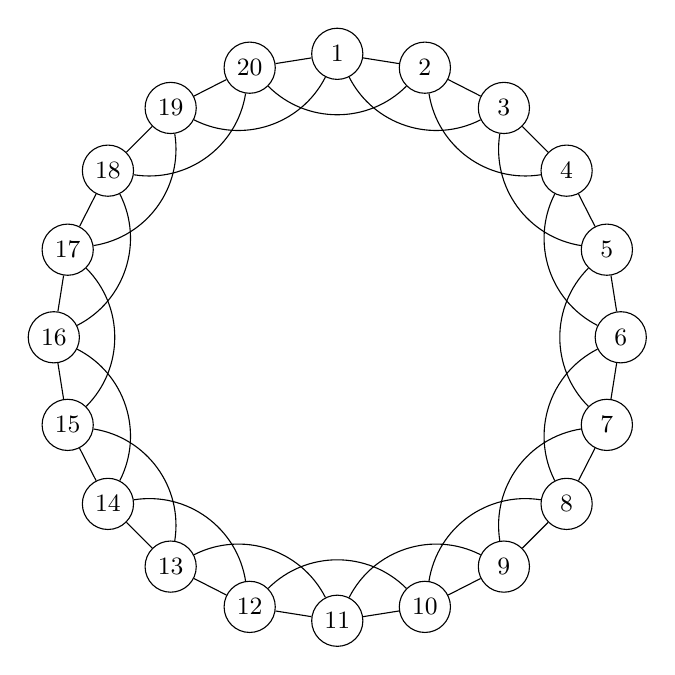
\begin{tikzpicture}[scale=1.0]
    \foreach \i in {1,...,20} {
        \node[draw, circle, inner sep=0.5pt, minimum size=6.5mm]
            (N\i) at ({90-(\i-1)*18}:3.6) {\small \i};
    }
    \foreach \i in {1,...,20} {
        \pgfmathtruncatemacro{\j}{mod(\i,20)+1}
        \pgfmathtruncatemacro{\k}{mod(\i+1,20)+1}
        \draw (N\i) -- (N\j);
        \draw (N\i) to[bend right=45] (N\k);
    }
\end{tikzpicture}
\end{center}

Work outward from person 1 in layers: first everyone one handshake away, then
everyone reachable from those, and so on. Fill in the counts.

\begin{center}
\begin{tabular}{|l|p{1.6cm}|p{1.6cm}|p{1.6cm}|p{1.6cm}|p{1.6cm}|}
\hline
Handshakes & 1 & 2 & 3 & 4 & 5 \\
\hline
How many people & & & & & \\[0.5cm]
\hline
\end{tabular}
\end{center}

The counts must add up to \underline{\hspace{1.5cm}}. Do they?

\vspace{1em}

\begin{minipage}{\textwidth}
{\bf Question 4}:
Fill in the ledger for that single moved friendship.

\begin{center}
{\small
\begin{tabular}{|l|p{2.6cm}|p{2.6cm}|p{2.2cm}|}
\hline
 & Before & After & Change (\%) \\
\hline
Friendships changed & --- & 1 out of 40 & \\[0.4cm]
\hline
Avg.\ handshakes from person 1 & & & \\[0.4cm]
\hline
Farthest person from 1 & & & \\[0.4cm]
\hline
Triangles in town & & & \\[0.4cm]
\hline
\end{tabular}
}
\end{center}
\end{minipage}

For the triangle row, you do not need to recount the town. Ask instead: which
triangles used the edge 1--2, and does the new edge 1--11 create any?

\begin{enumerate}
    \item Triangles killed by removing 1--2: \underline{\hspace{1.5cm}} \quad
          Triangles created by adding 1--11: \underline{\hspace{1.5cm}}
    \item You changed 2.5\% of the friendships. Which of the two quantities ---
          distance or triangles --- moved by much more than 2.5\%?

          \underline{\hspace{\textwidth}}

    \item Why is the new edge so much better at shortening paths than the old
          edge 1--2 was? Answer in terms of what each edge lets you skip.

          \underline{\hspace{\textwidth}}
\end{enumerate}

\clearpage

\section*{Part 3: Turning the dial}

Now do it the way the model does. Go through all forty friendships one at a
time, and with probability $p$ move that friendship to a randomly chosen
person. $p = 0$ leaves the town untouched; $p = 1$ scrambles it completely.

{\bf Question 5}:
Pick any one triangle in the original town.

\begin{enumerate}
    \item How many friendships does it consist of? \underline{\hspace{1.5cm}}
    \item That triangle is still there after the rewiring only if

          \underline{\hspace{\textwidth}}
    \item So the chance it survives is \underline{\hspace{3cm}}, and therefore
          the town's clustering after rewiring is

          \[
          C(p) \;=\; C(0) \times \underline{\hspace{3cm}}
          \]
    \item Evaluate:

          $C(0.01) = $ \underline{\hspace{2cm}} \quad
          $C(0.1) = $ \underline{\hspace{2cm}} \quad
          $C(0.5) = $ \underline{\hspace{2cm}}
\end{enumerate}

{\bf Question 6}:
Now the other quantity. At $p = 0.01$, how many of the forty friendships get
moved, on average? \underline{\hspace{2cm}}

From Question 4 you know what one moved friendship does. So:

\begin{enumerate}
    \item Roughly how many people does \emph{one} shortcut bring closer?
          \underline{\hspace{3cm}}
    \item Roughly how many triangles does \emph{one} moved friendship destroy?
          \underline{\hspace{3cm}}
    \item One of these two effects is felt by the whole town, the other only
          near the edge that moved. Which is which, and why does that make the
          two curves fall at completely different values of $p$?

          \underline{\hspace{\textwidth}}

          \underline{\hspace{\textwidth}}
\end{enumerate}

\clearpage

{\bf Question 7}:
Sketch both curves on the same axes: clustering as a fraction of its starting
value, and average handshakes as a fraction of its starting value. The
horizontal axis multiplies by ten at each tick.

\begin{center}
\begin{tikzpicture}
    \draw[->] (0,0) -- (10,0) node[right] {\small $p$};
    \draw[->] (0,0) -- (0,6.2) node[above] {\small fraction of value at $p=0$};
    \foreach \x/\lab in {0/0.001, 3/0.01, 6/0.1, 9/1} {
        \draw (\x,-0.1) -- (\x,0.1) node[below=4pt] {\small \lab};
    }
    \draw (-0.1,6) -- (0.1,6) node[left=6pt] {\small 1};
    \draw (-0.1,3) -- (0.1,3) node[left=6pt] {\small 0.5};
    \draw[dashed] (0,6) -- (10,6);
\end{tikzpicture}
\end{center}

Shade the band of $p$ where the town has short chains \emph{and} still keeps
most of its triangles. Then answer: is that band narrow, so that a town would
have to be tuned carefully to land in it, or wide enough that almost any real
town falls in by accident?

\underline{\hspace{\textwidth}}

\clearpage

\section*{Part 4: The number that lies}

You built $\sigma$ yourself on the previous sheet: how much more clustered the
town is than chance, divided by how much longer its chains are than chance.

\begin{center}
\begin{tcolorbox}[width=0.85\textwidth, colback=white]
For a coin-flip town of $n$ people with $\langle k \rangle$ friends each:
clustering $\approx \langle k \rangle / (n-1)$ and average handshakes
$\approx \ln n / \ln \langle k \rangle$.

Useful values: $\ln 4 \approx 1.4$, \; $\ln 20 \approx 3.0$, \;
$\ln 10{,}000 \approx 9.2$.
\end{tcolorbox}
\end{center}

\begin{minipage}{\textwidth}
{\bf Question 8}:
Compute $\sigma$ for Ringville \emph{before} any rewiring --- the plain ring you
measured in Part 1, with $p = 0$.

\begin{center}
\begin{tabular}{|l|p{2.6cm}|p{2.6cm}|p{2.2cm}|}
\hline
 & Ringville ($p=0$) & Coin-flip town & Ratio \\
\hline
Clustering & & & \\[0.4cm]
\hline
Avg.\ handshakes & & & \\[0.4cm]
\hline
\end{tabular}
\end{center}

\vspace{0.5em}

$\sigma = $ \underline{\hspace{3cm}}

\vspace{0.8em}

Is it above 1? \underline{\hspace{1.5cm}} \quad
But this town has no shortcuts at all. What has just gone wrong?

\underline{\hspace{\textwidth}}
\end{minipage}

\vspace{2em}

\begin{minipage}{\textwidth}
{\bf Question 9}:
Maybe the trouble is that twenty is a small town. Test that. Keep the same ring
rule --- everyone knows two neighbors on each side --- but let the town have
$10{,}000$ people. You do not need exact numbers; a rough value for each cell is
enough.

\begin{center}
\begin{tabular}{|l|p{2.4cm}|p{2.4cm}|p{2.4cm}|}
\hline
 & $n = 20$ & $n = 10{,}000$ & Grows or shrinks? \\
\hline
Clustering of the ring & & & \\[0.4cm]
\hline
Clustering of coin-flip town & & & \\[0.4cm]
\hline
Avg.\ handshakes, ring & & & \\[0.4cm]
\hline
Avg.\ handshakes, coin-flip & & & \\[0.4cm]
\hline
$\sigma$ & & & \\[0.4cm]
\hline
\end{tabular}
\end{center}
\end{minipage}

(For the ring, a person's average distance is about $n/8$ --- convince yourself
from the table in Question 2 before you use it.)

\begin{enumerate}
    \item As the ring town grows, does $\sigma$ approach 1, stay put, or run
          away? \underline{\hspace{3cm}}
    \item So what does ``$\sigma > 1$'' actually certify?

          \underline{\hspace{\textwidth}}
\end{enumerate}

{\bf Question 10}:
A paper lands on your desk. It reports $\sigma = 2.3$ for a brain network and
concludes it is a small world.

\begin{enumerate}
    \item Name two things the paper must tell you before that number means
          anything.

          \underline{\hspace{\textwidth}}

    \item $\sigma$ compares the network to a coin-flip town only. From
          Questions 8 and 9 you know why that is not enough. Propose a second
          comparison that would have caught the problem, and say what value
          your new test should give for a plain ring.

          \underline{\hspace{\textwidth}}

          \underline{\hspace{\textwidth}}
\end{enumerate}

\end{document}
